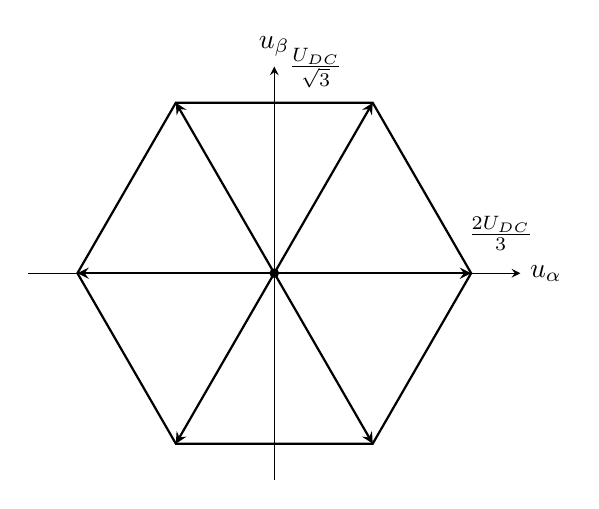
\begin{tikzpicture}[scale=2.5, >=stealth]

    \def\V{1}

    % axis
    \draw[->] (-1.25*\V,0) -- (1.25*\V,0)
        node[right] {$u_\alpha$};
    \draw[->] (0,-1.05*\V) -- (0,1.05*\V)
        node[above] {$u_\beta$};

    % hexagon
    \draw[thick]
        (0:\V)
        -- (60:\V)
        -- (120:\V)
        -- (180:\V)
        -- (240:\V)
        -- (300:\V)
        -- cycle;

    % vectors
    \foreach \angle/\label in {
        0,
        60,
        120,
        180,
        240,
        300
    }{
        \draw[->, thick]
            (0,0) -- (\angle:\V)
            node[pos=1.15] {};
    }

    \fill (0,0) circle (0.7pt);
	\node (node1) at (0.21,1.04) {$\frac{U_{DC}}{\sqrt{3}}$};
	\node (node2) at (1.15,0.2) {$\frac{2U_{DC}}{{3}}$};
\end{tikzpicture}